% fov_rt_et_CONTRIBUTION.tex

\section{Contribution}

\begin{figure*}
\parbox{.5\linewidth}{%
\centering%
\caption{Non-foveated ray tracing.}
\label{fig:histogram_non-foveated}
\input{gnu_non-foveated.tex} % \resizebox{1.0\linewidth}{!}{\input{gnu_non-foveated.tex}}
}
\hfill%
\parbox{.5\linewidth}{%
\centering%
\caption{Foveated ray tracing.}
\label{fig:histogram_foveated}
\input{gnu_foveated.tex} % \resizebox{1.0\linewidth}{!}{\input{gnu_foveated.tex}}
}
\end{figure*}

\begin{table*}[bp]
\parbox{.5\linewidth}{
\centering
\begin{tabular}{l|llll}
Stage & Avg. & Std. & Min. & Max.     \\ \hline
Gen. Rays     &     &     &     &     \\
Intersect     &     &     &     &     \\
Color         &     &     &     &    
\end{tabular}
\caption{Tabular 1.}
\label{tab:tabular1}}
\hfill
\parbox{.5\linewidth}{
\centering
\begin{tabular}{l|llll}
Stage & Avg. & Std. & Min. & Max.     \\ \hline
Gen. Rays     &     &     &     &     \\
Intersect     &     &     &     &     \\
Color         &     &     &     &    
\end{tabular}
\caption{Tabular 2.}
\label{tab:tabular2}}
\end{table*}

The ray tracing renderer devised for the purpose of this study adheres to the model presented by Garc{\'i}a et al.: devised in DirectCompute using C$++$.
The algorithm renders the scene with the help of three distinct steps that compiles a number of rays equal to that of the application window resolution, performs intersections tests on each ray with scene geometry to establish the closest intersected geometry, and finally draws the scene to the framebuffer using scene lights- and geometry in order to establish what areas of the scene are in shadow.
The ray tracing algorithm is presented as pseudocode in algorithm \ref{algrt}.
Note that some elements of the algorithm are not featured in-pseudo-code, such as the comparison of closest intersected scene geometry, in order to keep the code short and concise.

\begin{algorithm}
\begin{algorithmic}[1]
\Procedure{raytrace}{$rays, reflCnt$}
\caption{Ray tracing algorithm}\label{algrt}
\State $rays\gets$\Call{GenRays}{screen, frustum}
\While{$reflCnt>0$}
\ForAll{$rays$}\Comment{for each pixel}
\If {\Call{intersects}{ray, objs}}
    \State $obj\gets objs$
\EndIf
%\Require $obj$ % If you're to be entirely precise.
\ForAll{$lights$}
\State $color\gets$\Call{Shadow}{ray, obj}
\State $color\gets$\Call{Lighting}{obj}
\EndFor
\State $backbuffer\gets color$
\EndFor
\State $reflCnt\gets reflCnt - 1$
\EndWhile
\EndProcedure
\end{algorithmic}
\end{algorithm}

In order to optimize this algorithm to make it run sufficiently fast on the platform at hand we made use of a Tobii EyeX Dev Kit to establish where on the screen the observer is focusing his or her gaze.
Using this information, we may render only parts of the application window - where the user has his or her gaze fixation - at full resolution; rendering those areas of the window in the user's peripheral vision at a lower resolution.
Since, as described in algorithm \ref{algrt}, the total number of computed rays is based off the texel grid of the framebuffer this may drastically reduce the number of rays required to render a scene.

\subsection{Hardware}
For the purpose of this experiment, we make use of the Tobii EyeX Devkit Controller, which is a consumer-level corneal-reflection eye tracking device, which may the position the gaze of an oberserver on a computer screen.
The EyeX controller, while still a developer's prototype variant, is a fairly competent device; the consumer version expected to be released later this year.

The experiment is performed on a Windows~8.1 system with the following specifications:
\begin{itemize}
\setlength\itemsep{0em}
\item Intel Q9550 Quad Core 2.83GHz
\item ATI Radeon HD 5800
\end{itemize}

For the screen, we use a $23''$ $510$mm~$\times$~$287$mm Samsung~Syncmaster~$2343$ monitor, beneath which the eye tracking device is placed for the duration of the experiment.

\subsection{Software}
For retrieval of gaze positional data and communication with the eye tracking device, we utilize the Tobii C/C$++$~SDK.

In order to achieve varying levels of quality - or resolution - in the field-of-vision, the rendering process is subdivided into a number of 'FOV's (short for fovea, parafovea, etc.); each it's own render target.
Using an arbitrary of number these FOVs, we may vary the quality of the rendered scene accross the user's field of vision.
For the purpose of this study, although FOVs for both foveal-, parafoveal-, and peripheral vision have been prototyped, we limit the variance in quality to that of parafoveal and peripheral vision.
Thus, we render the scene at two different resolutions during the experiment; corresponding to parafoveal- and peripheral vision.

This is due to the EyeX controller device.
Being a consumer-level developer's kit, the device tracking may bring about a jittery render target when the designated area is as small as $2$\degree\ (human foveal vision) of the observer's view.
As this is considerably less noticable with a larger area (giving the eye tracking device more time to garner gaze positional data when the user moves his or her eyes); rendering the entirety of the parafoveal vision (5\degree ) at high quality was deemed more appropriate.
After all, the purposes of foveated rendering is to reduce computational complexity whilst maintaining percieved scene quality.

For our setup, the observer is positioned 700mm from the screen (which is the distance relayed appropriate by the device).
The application window resolution is that of $1152\times 1152$, a resolution chosen due to it being the highest our system setup could display whilst keeping the resolution square.
A $5$\degree\ parafovea thus bring about an area of roughly $31$mm$\times $$31$mm, which represents, for the utilized screen, roughly $123\times 123$~pixels; a small percentage of the application window resolution.
Note, however, that this component would be considerably smaller should the application run at even higher resolutions.
In fact, presuming the same system setup and distance to the screen, the pixel resolution within the observer's foveal vision should remain constant.

For the peripheral vision, or the low-quality render target, we chose to render the scene at only a fourth of the full-resolution.
Accordingly, our rendering algorithm is performed in an additional two steps; wherein the scene is rendered at full-resolution in a grid of only $123\times 123$ pixels, while the rest of the framebuffer is rendered at a fourth of full-resolution and subsequently upscaled to fit the application window.
The high-resolution parafoveal framebuffer is then copied onto the screen framebuffer at the location where the observer is currently focusing his or her gaze.

\begin{figure}[p]
  \centering
  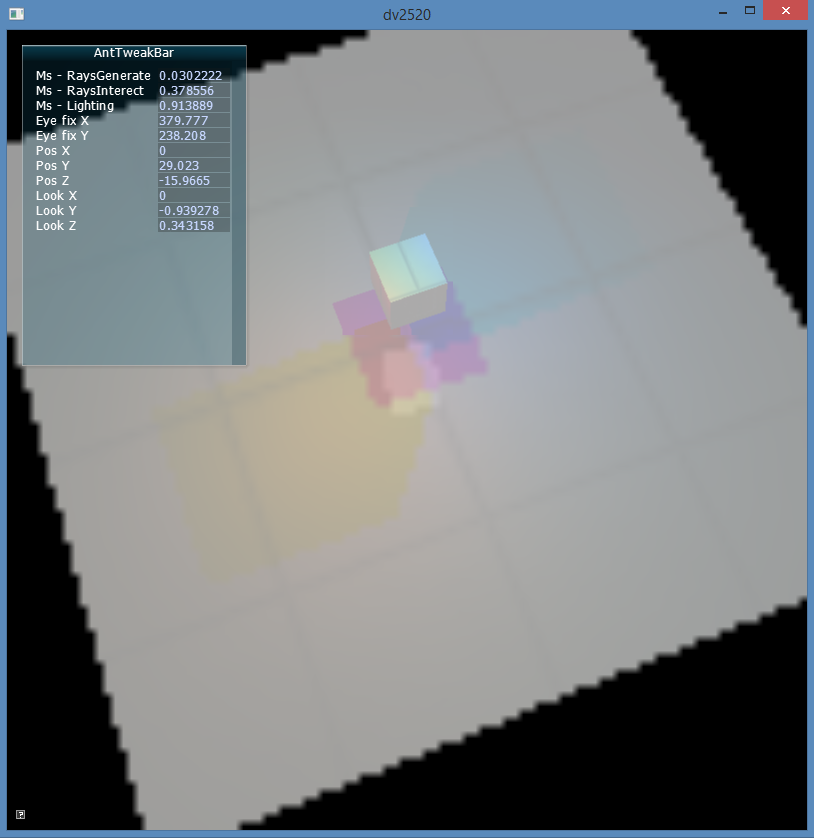
\includegraphics[width=1.0\linewidth]{img/fov_rt_et.png}
  \caption{An $800\times 800$ foveated scene. The observer's gaze is positioned on the cube. Note that the surrounding scenery, including the cube's reflection in the plane, is rendered at a lower resolution. This particular scene, on the contrary to the experiment, renders the peripheral areas in an eighth of the full-resolution in order to make the foveated effect more prominent and noticable for the sake of visualization.}
  \label{fig:fov}
\end{figure}
